\chapter{UART Serial Communication}

\section*{Learning Objectives}
After completing this experiment, you will be able to:
\begin{itemize}[nosep]
  \item Understand the principles of asynchronous serial communication using UART.
  \item Differentiate between synchronous and asynchronous communication protocols.
  \item Configure UART modules on the TM4C123 microcontroller for serial data transmission.
  \item Calculate and configure baud rate divisors for different communication speeds.
  \item Implement GPIO alternate function configuration for UART pins.
  \item Transmit and receive data through UART using polling and FIFO buffers.
  \item Create a reusable UART driver library with initialization, transmit, and receive functions.
  \item Interface with a PC terminal application for debugging and user interaction.
  \item Implement string-based communication protocols for command processing.
\end{itemize}

\section*{Experiment Overview}
Serial communication is one of the most fundamental methods for data exchange between microcontrollers and external devices. The Universal Asynchronous Receiver-Transmitter (UART) is a widely-used hardware communication protocol that enables simple, bidirectional, full-duplex serial data transmission without requiring a shared clock signal between devices.

\noindent UART is particularly valuable in embedded systems because of its simplicity, robustness, and widespread support across microcontrollers, sensors, GPS modules, Bluetooth modules, and debugging interfaces. Unlike synchronous protocols (SPI, I²C), UART does not need a clock line — both devices independently use agreed-upon timing parameters (baud rate) to synchronize data transmission.

\noindent The TM4C123 microcontroller features eight UART modules (UART0-UART7), each capable of supporting standard baud rates from 300 bps to 5 Mbps. UART0 is commonly used for debugging and communication with PC terminal applications through a USB-to-serial converter integrated into the TM4C123 LaunchPad.

\noindent In this experiment, you will:
\begin{itemize}[nosep]
  \item Learn the fundamentals of UART frame structure, timing, and baud rate calculation.
  \item Understand the role of UART hardware registers and FIFOs.
  \item Configure GPIO pins for UART alternate function (AFSEL, PCTL).
  \item Implement initialization routines for UART0 with specific baud rates and data formats.
  \item Transmit characters and strings from the microcontroller to a PC terminal.
  \item Receive characters and strings from a PC terminal with echo functionality.
  \item Debug embedded applications using serial output for status messages and variable monitoring.
\end{itemize}

By the end of this lab, you will be proficient in UART configuration and communication, enabling you to interface the TM4C123 with PCs, sensors, and other microcontrollers for data exchange and debugging.

\newpage
\etocsetnexttocdepth{subsubsection}
\localtableofcontents
\bigskip
\newpage

\section{Theoretical Background}

\subsection{UART Communication Fundamentals}

UART (Universal Asynchronous Receiver-Transmitter) is a hardware communication protocol that converts parallel data from a microcontroller's bus into serial format for transmission and vice versa for reception.

\subsubsection{Synchronous vs. Asynchronous Communication}

\paragraph{Synchronous Communication}
\begin{itemize}[nosep]
  \item \textbf{Shared clock}: Transmitter and receiver use a common clock signal (e.g., SPI's SCK, I²C's SCL)
  \item \textbf{Advantages}: Higher data rates, precise timing, simpler framing
  \item \textbf{Disadvantages}: Requires additional clock line, limited cable length due to clock skew
\end{itemize}

\paragraph{Asynchronous Communication (UART)}
\begin{itemize}[nosep]
  \item \textbf{No shared clock}: Each device uses its own independent clock
  \item \textbf{Timing synchronization}: Uses start/stop bits and agreed-upon baud rate
  \item \textbf{Advantages}: Only 2 wires needed (TX, RX), longer cable lengths, simpler hardware
  \item \textbf{Disadvantages}: Lower maximum data rates, requires precise clock accuracy, overhead from start/stop bits
\end{itemize}

\subsubsection{UART Data Frame Structure}

A UART transmission consists of a series of frames, each containing:

\begin{enumerate}[nosep]
  \item \textbf{Idle State}: Line held HIGH (logic 1) when no data is being transmitted
  \item \textbf{Start Bit}: A single LOW (logic 0) bit signals the beginning of a frame
  \item \textbf{Data Bits}: 5 to 9 bits of actual data (typically 8 bits for byte transmission)
  \item \textbf{Parity Bit} (optional): Even, odd, or no parity for error detection
  \item \textbf{Stop Bits}: 1, 1.5, or 2 HIGH bits marking the end of the frame
\end{enumerate}

\begin{figure}[H]
\centering
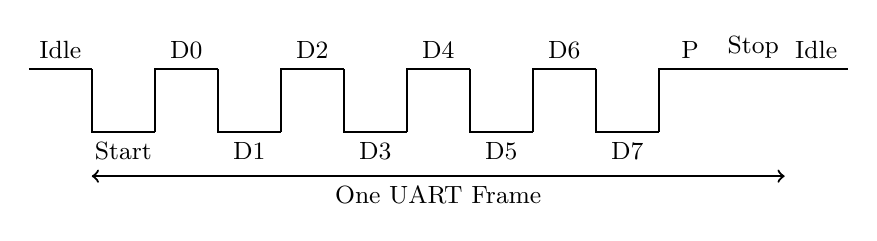
\begin{tikzpicture}[scale=0.8]
  % Idle state
  \draw[thick] (0,1) -- (1,1) node[midway,above] {\small Idle};
  
  % Start bit
  \draw[thick] (1,1) -- (1,0) -- (2,0) node[midway,below] {\small Start};
  
  % Data bits
  \draw[thick] (2,0) -- (2,1) -- (3,1) node[midway,above] {\small D0};
  \draw[thick] (3,1) -- (3,0) -- (4,0) node[midway,below] {\small D1};
  \draw[thick] (4,0) -- (4,1) -- (5,1) node[midway,above] {\small D2};
  \draw[thick] (5,1) -- (5,0) -- (6,0) node[midway,below] {\small D3};
  \draw[thick] (6,0) -- (6,1) -- (7,1) node[midway,above] {\small D4};
  \draw[thick] (7,1) -- (7,0) -- (8,0) node[midway,below] {\small D5};
  \draw[thick] (8,0) -- (8,1) -- (9,1) node[midway,above] {\small D6};
  \draw[thick] (9,1) -- (9,0) -- (10,0) node[midway,below] {\small D7};
  
  % Parity bit
  \draw[thick] (10,0) -- (10,1) -- (11,1) node[midway,above] {\small P};
  
  % Stop bit
  \draw[thick] (11,1) -- (12,1) node[midway,above] {\small Stop};
  
  % Idle again
  \draw[thick] (12,1) -- (13,1) node[midway,above] {\small Idle};
  
  % Labels
  \draw[<->,thick] (1,-0.7) -- (12,-0.7);
  \node at (6.5,-1) {\small One UART Frame};
\end{tikzpicture}
\caption{UART Frame Structure (8 data bits, 1 parity bit, 1 stop bit)}
\end{figure}

\noindent
\textbf{Common UART Configuration: 8N1}
\begin{itemize}[nosep]
  \item 8 data bits
  \item No parity (N)
  \item 1 stop bit
  \item Most widely used configuration for simplicity and efficiency
\end{itemize}

\subsubsection{Baud Rate}

The \textbf{baud rate} is the rate at which symbols (bits) are transmitted per second, measured in bits per second (bps). Common baud rates include:

\begin{itemize}[nosep]
  \item \textbf{9600 bps}: Slow, highly reliable, long cable lengths
  \item \textbf{115200 bps}: Fast, common for debugging and short cables
  \item \textbf{Other rates}: 4800, 19200, 38400, 57600, 230400, 460800, 921600 bps
\end{itemize}

\noindent
Both transmitter and receiver must use the \textit{exact same} baud rate. Even small differences (> 2-3\%) can cause communication errors due to timing drift over the duration of a frame.

\subsubsection{Full-Duplex Communication}

UART supports \textbf{full-duplex} communication, meaning data can be transmitted and received simultaneously on separate lines:
\begin{itemize}[nosep]
  \item \textbf{TX (Transmit)}: Output pin for sending data
  \item \textbf{RX (Receive)}: Input pin for receiving data
  \item \textbf{Connection}: TX of device A connects to RX of device B, and vice versa
  \item \textbf{Ground}: Shared ground reference is essential for proper voltage level detection
\end{itemize}

\subsection{TM4C123 UART Architecture}

The TM4C123 microcontroller includes eight UART modules (UART0-UART7) with advanced features:

\subsubsection{UART Features}
\begin{itemize}[nosep]
  \item \textbf{Baud rate generation}: Programmable from 300 bps to 5 Mbps
  \item \textbf{Data formats}: 5, 6, 7, 8, or 9 data bits
  \item \textbf{Parity}: Even, odd, or no parity
  \item \textbf{Stop bits}: 1 or 2 stop bits
  \item \textbf{FIFOs}: 16-byte transmit and receive FIFOs with programmable trigger levels
  \item \textbf{Interrupts}: Transmit, receive, overrun, framing error, parity error, break detection
  \item \textbf{DMA support}: Direct Memory Access for high-throughput transfers
  \item \textbf{IrDA and 9-bit modes}: Advanced communication modes
\end{itemize}

\subsubsection{UART Pin Mapping}

Each UART module is mapped to specific GPIO pins through alternate function configuration:

\begin{table}[H]
\centering
\small
\renewcommand{\arraystretch}{1.2}
\begin{tabular}{llll}
\toprule
\textbf{UART Module} & \textbf{TX Pin} & \textbf{RX Pin} & \textbf{Notes} \\
\midrule
UART0 & PA1 & PA0 & Connected to USB-to-serial on LaunchPad \\
UART1 & PB1 & PB0 & Available on expansion headers \\
UART2 & PD7 & PD6 & Available on expansion headers \\
UART3 & PC7 & PC6 & Available on expansion headers \\
UART4 & PC5 & PC4 & Available on expansion headers \\
UART5 & PE5 & PE4 & Available on expansion headers \\
UART6 & PD5 & PD4 & Available on expansion headers \\
UART7 & PE1 & PE0 & Available on expansion headers \\
\bottomrule
\end{tabular}
\caption{TM4C123 UART Pin Assignments}
\end{table}

\noindent
In this experiment, we use \textbf{UART0} (PA0/PA1) because it is directly connected to the on-board USB-to-serial converter, allowing easy communication with a PC terminal without additional hardware.

\subsection{UART Registers}

The UART modules are controlled through memory-mapped registers. Key registers include:

\subsubsection{UARTDR — Data Register}
\noindent\textbf{Register:} \texttt{UARTx->DR} — UART Data (\texttt{Base + 0x000})

\noindent
The Data Register is used for both transmitting and receiving data:
\begin{itemize}[nosep]
  \item \textbf{Write}: Places data in the transmit FIFO (bits 7:0 contain the byte to transmit)
  \item \textbf{Read}: Retrieves data from the receive FIFO (bits 7:0 contain the received byte)
  \item \textbf{Error flags} (bits 11:8 on read): Framing Error (FE), Parity Error (PE), Break Error (BE), Overrun Error (OE)
\end{itemize}

\subsubsection{UARTFR — Flag Register}
\noindent\textbf{Register:} \texttt{UARTx->FR} — UART Flag Register (\texttt{Base + 0x018})

\noindent
The Flag Register provides status information about the UART:

\begin{table}[H]
\centering
\small
\renewcommand{\arraystretch}{1.2}
\begin{tabular}{clp{7cm}}
\toprule
\textbf{Bit} & \textbf{Name} & \textbf{Description} \\
\midrule
0 & CTS & Clear To Send (hardware flow control, not commonly used) \\
3 & BUSY & UART busy transmitting data \\
4 & RXFE & Receive FIFO Empty (1 = empty, 0 = data available) \\
5 & TXFF & Transmit FIFO Full (1 = full, wait before writing) \\
6 & RXFF & Receive FIFO Full \\
7 & TXFE & Transmit FIFO Empty (1 = empty, transmission complete) \\
\bottomrule
\end{tabular}
\caption{UARTFR Register Bits}
\end{table}

\subsubsection{UARTIBRD and UARTFBRD — Baud Rate Divisors}
\noindent\textbf{Registers:} \texttt{UARTx->IBRD} and \texttt{UARTx->FBRD}

\noindent
The baud rate is determined by dividing the UART clock by a divisor:

\[
\text{Baud Rate} = \frac{f_{\text{UART clock}}}{16 \times (\text{IBRD} + \text{FBRD})}
\]

\noindent
Where:
\begin{itemize}[nosep]
  \item \textbf{IBRD}: Integer part of the baud rate divisor (16-bit value)
  \item \textbf{FBRD}: Fractional part of the baud rate divisor (6-bit value, represents fraction/64)
\end{itemize}

\noindent
\textbf{Calculation Steps:}
\begin{enumerate}[nosep]
  \item Calculate divisor: $\text{Divisor} = \frac{f_{\text{UART clock}}}{16 \times \text{Baud Rate}}$
  \item Integer part: $\text{IBRD} = \lfloor \text{Divisor} \rfloor$
  \item Fractional part: $\text{FBRD} = \text{round}((\text{Divisor} - \text{IBRD}) \times 64 + 0.5)$
\end{enumerate}

\noindent
\textbf{Example: 115200 baud at 50 MHz system clock}
\[
\text{Divisor} = \frac{50{,}000{,}000}{16 \times 115{,}200} = \frac{50{,}000{,}000}{1{,}843{,}200} \approx 27.126
\]
\[
\text{IBRD} = 27, \quad \text{FBRD} = \text{round}(0.126 \times 64 + 0.5) = \text{round}(8.564) = 8
\]

\subsubsection{UARTLCRH — Line Control Register}
\noindent\textbf{Register:} \texttt{UARTx->LCRH} — UART Line Control (\texttt{Base + 0x02C})

\noindent
The Line Control Register configures the frame format:

\begin{table}[H]
\centering
\small
\renewcommand{\arraystretch}{1.2}
\begin{tabular}{clp{6.5cm}}
\toprule
\textbf{Bits} & \textbf{Name} & \textbf{Description} \\
\midrule
0 & BRK & Send break (force TX low) \\
1 & PEN & Parity Enable (0 = no parity, 1 = parity enabled) \\
2 & EPS & Even Parity Select (0 = odd, 1 = even) \\
3 & STP2 & Two Stop Bits (0 = 1 stop bit, 1 = 2 stop bits) \\
4 & FEN & FIFO Enable (0 = disable FIFOs, 1 = enable FIFOs) \\
6:5 & WLEN & Word Length: 00 = 5 bits, 01 = 6 bits, 10 = 7 bits, 11 = 8 bits \\
7 & SPS & Stick Parity Select \\
\bottomrule
\end{tabular}
\caption{UARTLCRH Register Bits}
\end{table}

\noindent
\textbf{Common configuration (8N1 with FIFOs):}
\begin{lstlisting}[language=C]
UART0->LCRH = (0x3 << 5) | (1 << 4);  // 8 data bits, FIFOs enabled
// Or: UART0->LCRH = 0x60;
\end{lstlisting}

\subsubsection{UARTCTL — Control Register}
\noindent\textbf{Register:} \texttt{UARTx->CTL} — UART Control (\texttt{Base + 0x030})

\noindent
The Control Register enables/disables the UART and its transmit/receive functions:

\begin{table}[H]
\centering
\small
\renewcommand{\arraystretch}{1.2}
\begin{tabular}{clp{7cm}}
\toprule
\textbf{Bit} & \textbf{Name} & \textbf{Description} \\
\midrule
0 & UARTEN & UART Enable (0 = disable, 1 = enable) \\
8 & TXE & Transmit Enable (0 = disable TX, 1 = enable TX) \\
9 & RXE & Receive Enable (0 = disable RX, 1 = enable RX) \\
\bottomrule
\end{tabular}
\caption{UARTCTL Register Key Bits}
\end{table}

\noindent
\textbf{Enable UART with TX and RX:}
\begin{lstlisting}[language=C]
UART0->CTL = (1 << 0) | (1 << 8) | (1 << 9);  // Enable UART, TX, RX
// Or: UART0->CTL = 0x301;
\end{lstlisting}

\subsubsection{UARTCC — Clock Configuration}
\noindent\textbf{Register:} \texttt{UARTx->CC} — UART Clock Configuration (\texttt{Base + 0xFC8})

\noindent
Selects the clock source for the UART module:
\begin{itemize}[nosep]
  \item \texttt{0x0}: System clock (default and most common)
  \item \texttt{0x5}: PIOSC (16 MHz internal oscillator)
\end{itemize}

\subsection{UART Configuration Workflow}

The following steps configure UART0 for basic serial communication:

\begin{enumerate}[nosep]
  \item \textbf{Enable clocks}: Enable UART0 and GPIOA clocks in \texttt{SYSCTL->RCGCUART} and \texttt{SYSCTL->RCGCGPIO}
  \item \textbf{Wait for clock stabilization}: Check ready bits or insert delay
  \item \textbf{Disable UART}: Clear \texttt{UART0->CTL} during configuration
  \item \textbf{Configure GPIO for UART alternate function}:
    \begin{itemize}[nosep]
      \item Enable alternate function: \texttt{GPIOA->AFSEL |= 0x03} (PA0, PA1)
      \item Set port control: \texttt{GPIOA->PCTL |= 0x11} (UART function on PA0/PA1)
      \item Enable digital: \texttt{GPIOA->DEN |= 0x03}
    \end{itemize}
  \item \textbf{Set baud rate divisors}: Write \texttt{UART0->IBRD} and \texttt{UART0->FBRD}
  \item \textbf{Configure line control}: Set data bits, parity, stop bits, enable FIFOs in \texttt{UART0->LCRH}
  \item \textbf{Select clock source}: \texttt{UART0->CC = 0} (system clock)
  \item \textbf{Enable UART}: Set \texttt{UART0->CTL} to enable UART, TX, and RX
\end{enumerate}

\newpage
\section{Procedure}

\subsection{Example: Basic UART Driver Implementation}

The following code demonstrates a complete UART driver for UART0 with initialization, character/string transmission, and character/string reception.

\subsubsection{UART Header File}

\lstinputlisting[language=C, caption={UART driver header file (\texttt{uart.h})}]{snippets/uart/uart.h}

\subsubsection{UART Implementation File}

\lstinputlisting[language=C, caption={UART driver implementation (\texttt{uart.c})}]{snippets/uart/uart.c}

\subsubsection{Main Application}

\lstinputlisting[language=C, caption={Main application using UART driver (\texttt{main.c})}]{snippets/uart/main.c}

\subsection{Code Explanation}

\paragraph{UART Initialization}
The \texttt{UART0\_Init()} function configures UART0 for 115200 baud, 8N1 format with FIFOs enabled:
\begin{enumerate}[nosep]
  \item Enables UART0 and GPIOA clocks
  \item Configures PA0 (RX) and PA1 (TX) for UART alternate function using AFSEL, PCTL, and DEN
  \item Disables UART0 during configuration
  \item Sets baud rate divisors: IBRD = 27, FBRD = 8 for 115200 baud at 50 MHz
  \item Configures line control: 8 data bits (\texttt{WLEN = 0x3}), FIFOs enabled (\texttt{FEN = 1})
  \item Selects system clock as UART clock source
  \item Enables UART0 with transmit and receive functions
\end{enumerate}

\paragraph{Transmitting Data}
The \texttt{UART0\_WriteChar()} function sends a single character:
\begin{itemize}[nosep]
  \item Polls the TXFF flag (bit 5) in the FR register
  \item Waits while TXFF = 1 (transmit FIFO full)
  \item Writes character to DR register when FIFO has space
  \item Hardware automatically handles framing (start bit, data bits, stop bit)
\end{itemize}

\noindent
The \texttt{UART0\_WriteString()} function sends a null-terminated string by repeatedly calling \texttt{UART0\_WriteChar()}.

\paragraph{Receiving Data}
The \texttt{UART0\_ReadChar()} function receives a single character:
\begin{itemize}[nosep]
  \item Polls the RXFE flag (bit 4) in the FR register
  \item Waits while RXFE = 1 (receive FIFO empty)
  \item Reads character from DR register when data is available
  \item Masks to 8 bits (\texttt{0xFF}) to extract data byte
\end{itemize}

\noindent
The \texttt{UART0\_ReadString()} function reads characters until Enter (\texttt{\textbackslash r} or \texttt{\textbackslash n}), with optional echo.

\paragraph{Main Application}
The main program demonstrates:
\begin{enumerate}[nosep]
  \item UART initialization
  \item Sending a greeting message
  \item Echo loop: reading a string, echoing it back with a prefix
\end{enumerate}

\subsection{Using PuTTY for Serial Communication}

To interact with the TM4C123 via UART0, use a terminal emulator like PuTTY:

\begin{enumerate}[nosep]
  \item Download and install PuTTY from \url{https://www.putty.org/}
  \item Connect the TM4C123 LaunchPad to your PC via USB
  \item Open Windows Device Manager and find the COM port under ``Ports (COM \& LPT)'' (e.g., COM3)
  \item Launch PuTTY and configure:
    \begin{itemize}[nosep]
      \item Connection type: Serial
      \item Serial line: COMx (replace with your COM port)
      \item Speed: 115200 (or your configured baud rate)
    \end{itemize}
  \item Click ``Open'' to establish connection
  \item Type text and press Enter to send strings to the microcontroller
  \item View echoed responses and debug output
\end{enumerate}

\begin{figure}[H]
\centering
\includegraphics[width=0.6\textwidth]{resources/putty.png}
\caption{PuTTY Serial Configuration}
\label{fig:putty_config}
\end{figure}

\noindent
\textbf{Tip}: Enable ``Local echo'' in PuTTY settings (Terminal → Line discipline options) to see your typed characters even before the microcontroller echoes them back.

\newpage
\subsection{Tasks}

\subsubsection{Task 1: LED Control via UART Commands}

Write a program that receives single-character commands via UART to control the on-board LEDs.

\paragraph{Requirements:}
\begin{itemize}[nosep]
  \item Initialize UART0 and configure GPIO Port F for LEDs (PF1/Red, PF2/Blue, PF3/Green)
  \item Receive single characters via UART0
  \item Implement command processing:
    \begin{itemize}[nosep]
      \item \texttt{'r'} or \texttt{'R'}: Toggle RED LED
      \item \texttt{'b'} or \texttt{'B'}: Toggle BLUE LED
      \item \texttt{'g'} or \texttt{'G'}: Toggle GREEN LED
      \item \texttt{'a'} or \texttt{'A'}: Turn all LEDs ON
      \item \texttt{'x'} or \texttt{'X'}: Turn all LEDs OFF
    \end{itemize}
  \item Echo back confirmation messages (e.g., ``RED LED toggled'')
  \item Send error message for unrecognized commands
\end{itemize}

\paragraph{Hint:}
\begin{lstlisting}[language=C]
char cmd = UART0_ReadChar();
switch (cmd) {
    case 'r':
    case 'R':
        GPIOF->DATA ^= (1 << 1);  // Toggle RED
        UART0_WriteString("RED LED toggled\r\n");
        break;
    // ... other cases
    default:
        UART0_WriteString("Unknown command\r\n");
}
\end{lstlisting}

\subsubsection{Task 2: ADC Value Monitoring}

Create a program that reads the on-board temperature sensor (or potentiometer) using ADC and continuously sends the values to a PC terminal.

\paragraph{Requirements:}
\begin{itemize}[nosep]
  \item Initialize UART0 for serial communication
  \item Initialize ADC0 to read the internal temperature sensor (ADC0 sequencer 3)
  \item Use a timer (SysTick or GPTM) to trigger ADC sampling every 1 second
  \item Convert ADC value to temperature in degrees Celsius using the formula:
    \[
    T_{\text{C}} = 147.5 - \frac{(\text{ADC\_Value} \times 3.3 \times 100)}{4096}
    \]
  \item Format and send the temperature reading via UART (e.g., ``Temp: 25.3 C'')
  \item Use \texttt{sprintf()} to format floating-point values into strings
\end{itemize}

\paragraph{Hint:}
\begin{lstlisting}[language=C]
#include <stdio.h>

char buffer[50];
float temp = 147.5 - ((adcValue * 3.3 * 100) / 4096.0);
sprintf(buffer, "Temperature: %.1f C\r\n", temp);
UART0_WriteString(buffer);
\end{lstlisting}

\subsubsection{Task 3: Simple Command-Line Interface}

Implement a simple command-line interface (CLI) that accepts multi-character commands and arguments.

\paragraph{Requirements:}
\begin{itemize}[nosep]
  \item Display a welcome message and prompt (``>'') after initialization
  \item Read complete strings (terminated by Enter) using \texttt{UART0\_ReadString()}
  \item Parse commands with arguments (e.g., ``LED RED ON'', ``DELAY 500'')
  \item Implement command processing:
    \begin{itemize}[nosep]
      \item \texttt{LED <color> <ON|OFF>}: Control specific LED
      \item \texttt{BLINK <color> <count>}: Blink LED specified number of times
      \item \texttt{STATUS}: Report current LED states
      \item \texttt{HELP}: Display available commands
    \end{itemize}
  \item Send confirmation or error messages
  \item Display prompt after each command execution
\end{itemize}

\paragraph{Hint:}
Use \texttt{strcmp()} and \texttt{strtok()} for string parsing:
\begin{lstlisting}[language=C]
#include <string.h>

char buffer[50];
UART0_ReadString(buffer, 50);

char *cmd = strtok(buffer, " ");
if (strcmp(cmd, "LED") == 0) {
    char *color = strtok(NULL, " ");
    char *state = strtok(NULL, " ");
    // Process LED command
} else if (strcmp(cmd, "STATUS") == 0) {
    // Report status
}
UART0_WriteString("> ");  // Display prompt
\end{lstlisting}

\subsection{Testing and Debugging}

\subsubsection{Common Issues and Solutions}

\paragraph{No output in terminal}
\begin{itemize}[nosep]
  \item \textbf{Cause}: Wrong COM port, incorrect baud rate, or UART not initialized
  \item \textbf{Solution}: Verify COM port in Device Manager, ensure baud rates match (115200), check UART initialization code
\end{itemize}

\paragraph{Garbled characters}
\begin{itemize}[nosep]
  \item \textbf{Cause}: Baud rate mismatch between microcontroller and terminal
  \item \textbf{Solution}: Recalculate IBRD and FBRD values, verify system clock frequency, ensure terminal baud rate matches code
\end{itemize}

\paragraph{Missing characters or corrupted data}
\begin{itemize}[nosep]
  \item \textbf{Cause}: FIFO overrun, insufficient processing speed, timing issues
  \item \textbf{Solution}: Enable FIFOs, process received data promptly, consider interrupt-driven reception for high data rates
\end{itemize}

\paragraph{Characters not echoing back}
\begin{itemize}[nosep]
  \item \textbf{Cause}: RX not configured, GPIO alternate function not set correctly
  \item \textbf{Solution}: Verify GPIOA->AFSEL, GPIOA->PCTL, GPIOA->DEN settings, ensure RXE bit is set in UART0->CTL
\end{itemize}

\subsubsection{Debugging Strategy}

\begin{enumerate}[nosep]
  \item \textbf{Test transmission first}: Send fixed strings to verify TX is working before implementing RX
  \item \textbf{Use LED indicators}: Toggle LEDs after UART initialization and during character transmission/reception
  \item \textbf{Verify clock configuration}: Ensure system clock is 50 MHz as expected
  \item \textbf{Check register values}: Use debugger to inspect UART registers (CTL, FR, IBRD, FBRD, LCRH)
  \item \textbf{Test with simple echo}: Start with single-character echo before implementing complex string processing
  \item \textbf{Monitor FIFO flags}: Check TXFF and RXFE flags to ensure proper FIFO operation
\end{enumerate}

\subsubsection{Advanced UART Features}

For more sophisticated applications, consider exploring:
\begin{itemize}[nosep]
  \item \textbf{Interrupt-driven I/O}: Use UART interrupts instead of polling for better CPU efficiency
  \item \textbf{DMA transfers}: Offload large data transfers to DMA controller
  \item \textbf{Hardware flow control}: Implement RTS/CTS for reliable high-speed communication
  \item \textbf{9-bit mode}: Support address/data distinction in multi-processor systems
  \item \textbf{LIN and IrDA modes}: Special communication protocols for automotive and infrared applications
\end{itemize}
